\documentclass[12pt, letterpaper]{report}
\usepackage{graphicx}
\usepackage{hyperref}
\usepackage{amssymb}
\usepackage{amsmath}
\usepackage{float}
\usepackage{mathtools}
\usepackage{enumitem}
\usepackage[margin=1in]{geometry}
\usepackage[figurename=Figura]{caption}
\title{Actividad: Problema Coulomb}
\author{Juan Pablo Guerrero Escudero A01706810}
\date{03 abril, 2024}
\begin{document}
\maketitle
\subsection*{Resolución del Problema}
\begin{figure}[H]
    \centering
    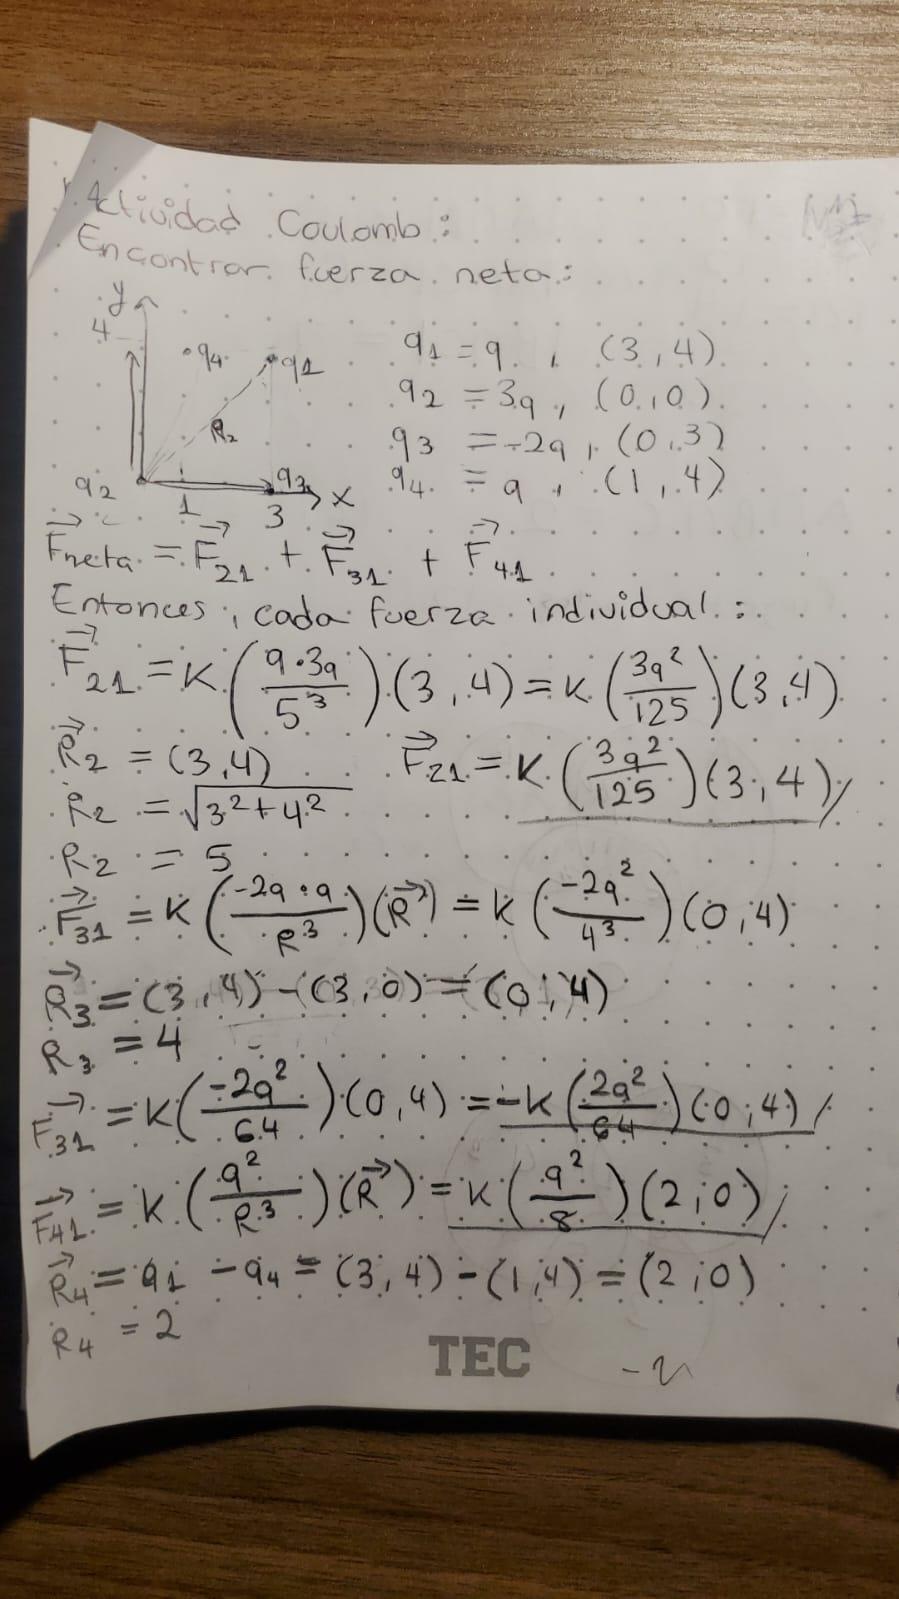
\includegraphics[height = 20cm]{2024-04-03_ProblemaCoulomb_1.jpeg}
    \caption{Primera página de solución}
\end{figure}
\begin{figure}[H]
    \centering
    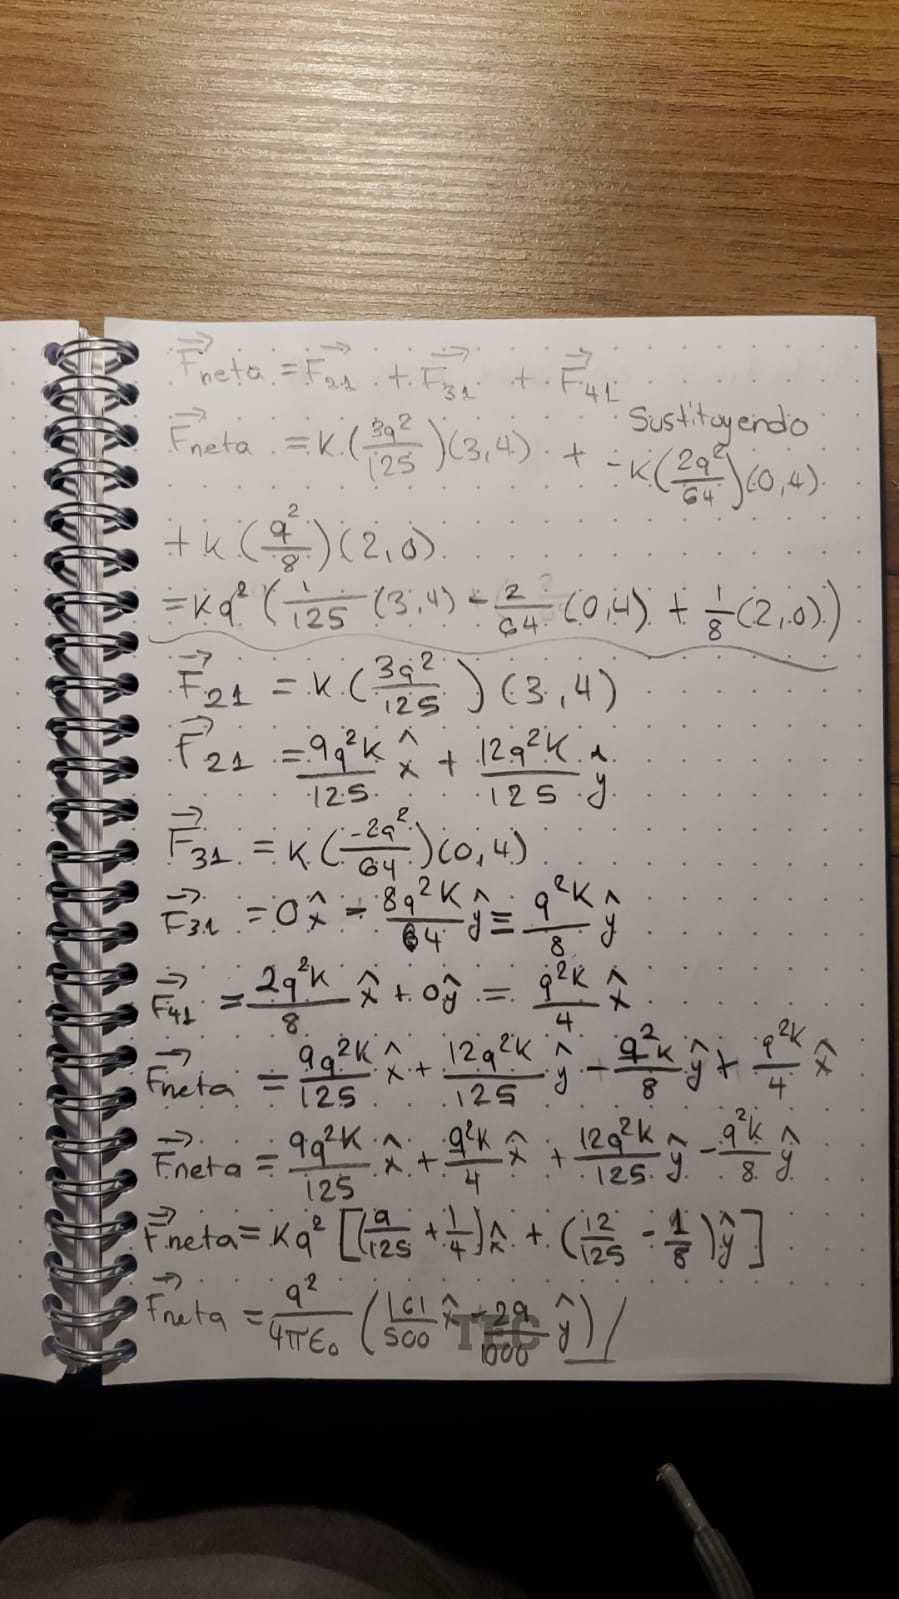
\includegraphics[height = 20cm]{2024-04-03_ProblemaCoulomb_2.jpeg}
    \caption{Segunda página de solución}
\end{figure}
\end{document}